\addcontentsline{toc}{subsection}{Area Under the Curve with RAM}
\subsection*{Area Under the Curve with RAM}
A train moves along a track at a steady rate of 75 miles per hour from 7 am to 9 am. What is the total distance traveled by the train? What if the train doesn't travel at a steady rate? Then how do you find the distance?
\vspace{\stretch{.6}}

Our goal is to calculate the area under a curve. We do that by breaking the area (which we cannot calculate) into rectangles (whose area we can calculate) and adding them together.

\begin{questions}
    
    \question Given $y=x^2$, what is the area under the curve from $x=0$ to $x=4$?
    
    \begin{minipage}[t]{0.3\linewidth}
        \begin{center}
        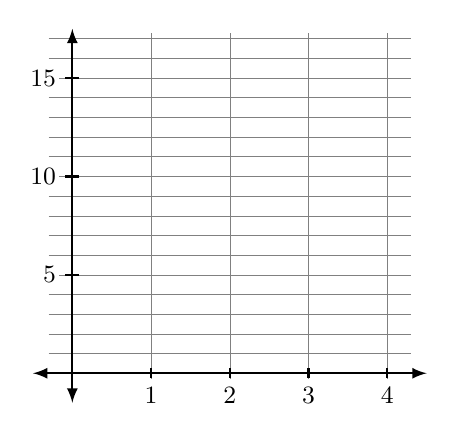
\begin{tikzpicture}[xscale=1,yscale=.25]
            \draw[step=1,style=help lines,] (-0.3,-.3) grid (4.3,17.3);
            \draw[latex-latex, thick] (-.5,0)--(4.5,0);
            \draw[latex-latex, thick] (0,-1.5)--(0,17.5);
            \foreach \x in {1,2,3,4}
                \draw[thick] (\x,7.5pt) -- (\x,-7.5pt) node [below=.7mm,fill=white,inner sep=1pt] {\small$\x$};
            \foreach \y in {5,10,15}
                \draw[thick] (2.5pt,\y) -- (-2.5pt,\y) node [left=.7mm,fill=white,inner sep=1pt] {\small$\y$};
        \end{tikzpicture}
        \end{center}
    \end{minipage}
    \hfill
    \begin{minipage}[t]{0.3\linewidth}
        \begin{center}
        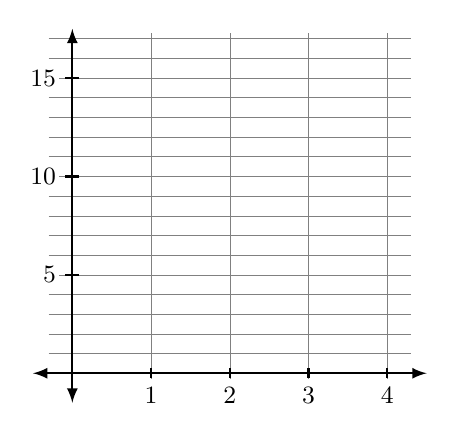
\begin{tikzpicture}[xscale=1,yscale=.25]
            \draw[step=1,style=help lines,] (-0.3,-.3) grid (4.3,17.3);
            \draw[latex-latex, thick] (-.5,0)--(4.5,0);
            \draw[latex-latex, thick] (0,-1.5)--(0,17.5);
            \foreach \x in {1,2,3,4}
                \draw[thick] (\x,7.5pt) -- (\x,-7.5pt) node [below=.7mm,fill=white,inner sep=1pt] {\small$\x$};
            \foreach \y in {5,10,15}
                \draw[thick] (2.5pt,\y) -- (-2.5pt,\y) node [left=.7mm,fill=white,inner sep=1pt] {\small$\y$};
        \end{tikzpicture}
        \end{center}
    \end{minipage}
    \hfill
    \begin{minipage}[t]{0.3\linewidth}
        \begin{center}
        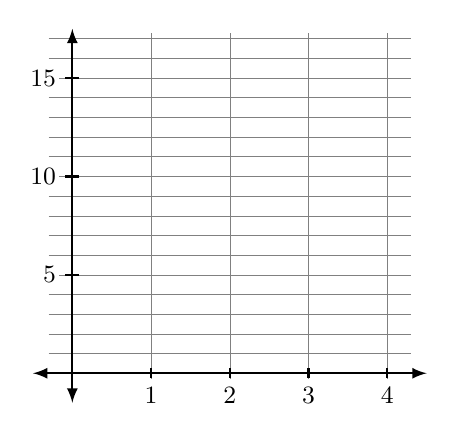
\begin{tikzpicture}[xscale=1,yscale=.25]
            \draw[step=1,style=help lines,] (-0.3,-.3) grid (4.3,17.3);
            \draw[latex-latex, thick] (-.5,0)--(4.5,0);
            \draw[latex-latex, thick] (0,-1.5)--(0,17.5);
            \foreach \x in {1,2,3,4}
                \draw[thick] (\x,7.5pt) -- (\x,-7.5pt) node [below=.7mm,fill=white,inner sep=1pt] {\small$\x$};
            \foreach \y in {5,10,15}
                \draw[thick] (2.5pt,\y) -- (-2.5pt,\y) node [left=.7mm,fill=white,inner sep=1pt] {\small$\y$};
        \end{tikzpicture}
        \end{center}
    \end{minipage}
    
    \vspace{\stretch{1}}
    
    \begin{center}
        \underline{RAM is the Rectangular Approximation Method}\\
        LRAM is the left hand values of $y$\\
        RRAM is the right hand values of $y$\\
        MRAM is the midpoint of L and R
    \end{center}
    
    \vspace{\stretch{.1}}
    
    \newpage
    
    \question Find the area between the $x$-axis and the curve $y=-x^2+2x+24$ using MRAM and 5 intervals (5 rectangles). MAKE A SKETCH along with your approximation.
    \vspace{\stretch{1}}
    
    
    \begin{minipage}[t]{0.55\linewidth}
    \question The table to the right shows the velocity of a model train engine moving along a track for 10 seconds. Estimate the distance traveled by the engine, using MRAM over 5 subintervals. Again, make a sketch!    
    \end{minipage}
    \hfill
    \begin{minipage}[t]{0.4\linewidth}
    \begin{longtable}[ht]{|C{2.25cm}|C{3cm}|}
        \hline
        Time (sec)\Tstrut\Bstrut & Velocity (in/sec)\Tstrut\Bstrut \\\hline
        $0$\Tstrut\Bstrut & $0$\Tstrut\Bstrut \\\hline
        $1$\Tstrut\Bstrut & $12$\Tstrut\Bstrut \\\hline
        $2$\Tstrut\Bstrut & $22$\Tstrut\Bstrut \\\hline
        $3$\Tstrut\Bstrut & $10$\Tstrut\Bstrut \\\hline
        $4$\Tstrut\Bstrut & $5$\Tstrut\Bstrut \\\hline 
        $5$\Tstrut\Bstrut & $13$\Tstrut\Bstrut \\\hline
        $6$\Tstrut\Bstrut & $11$\Tstrut\Bstrut \\\hline
        $7$\Tstrut\Bstrut & $6$\Tstrut\Bstrut \\\hline
        $8$\Tstrut\Bstrut & $2$\Tstrut\Bstrut \\\hline
        $9$\Tstrut\Bstrut & $6$\Tstrut\Bstrut \\\hline
        $10$\Tstrut\Bstrut & $0$\Tstrut\Bstrut \\\hline
    \end{longtable}    
    \end{minipage}
    

    
    
    \vspace{\stretch{.5}}
    
    \newpage
    
    \question Oil is leaking out of a tanker damaged at sea. The damage to the tanker is worsening as evidenced by the increased leakage each hour, recorded in the table below.
    \begin{parts}
        \part Give an upper and lower estimate of the total quantity of oil that has escaped over the 8 hours.
        \part The tanker continues to leak 720 gal/h after the first 8 hours. If the tanker originally contained 25,000 gallons of oil, approximately how many more hours will elapse in the worst case before all the oil has leaked? In the best case?
    \end{parts}
    
    
    \begin{longtable}[r]{|C{2cm}|C{3cm}|}
        \hline
        Time (h)\Tstrut\Bstrut & Leakage (gal/h)\Tstrut\Bstrut \\\hline
        $0$\Tstrut\Bstrut & $50$\Tstrut\Bstrut \\\hline
        $1$\Tstrut\Bstrut & $70$\Tstrut\Bstrut \\\hline
        $2$\Tstrut\Bstrut & $97$\Tstrut\Bstrut \\\hline
        $3$\Tstrut\Bstrut & $136$\Tstrut\Bstrut \\\hline
        $4$\Tstrut\Bstrut & $190$\Tstrut\Bstrut \\\hline 
        $5$\Tstrut\Bstrut & $265$\Tstrut\Bstrut \\\hline
        $6$\Tstrut\Bstrut & $369$\Tstrut\Bstrut \\\hline
        $7$\Tstrut\Bstrut & $516$\Tstrut\Bstrut \\\hline
        $8$\Tstrut\Bstrut & $720$\Tstrut\Bstrut \\\hline
    \end{longtable}    
    
    
    \hfill
    
    \vspace{\stretch{1}}
    
    \hfill
    
    \begin{longtable}[ht]{|C{1cm}|C{1cm}|C{1cm}|C{1cm}|C{1cm}|C{1cm}|}
        \hline
        $x$\Tstrut\Bstrut & $1$\Tstrut\Bstrut & $1.1$\Tstrut\Bstrut & $1.2$\Tstrut\Bstrut & $1.3$\Tstrut\Bstrut & $1.4$\Tstrut\Bstrut \\\hline
        $f'(x)$\Tstrut\Bstrut & $8$\Tstrut\Bstrut & $10$\Tstrut\Bstrut & $12$\Tstrut\Bstrut & $13$\Tstrut\Bstrut & $14.5$\Tstrut\Bstrut \\\hline
    \end{longtable}
    
    
    \question Use a Midpoint Riemann sum with two subintervals of equal length and values (directly above) from the table to approximate $\displaystyle\int_1^{1.4} f'(x)\,dx$.
    
    
    
\end{questions}


\newpage



\subsection*{Trapezoidal Rule}
\begin{tcolorbox}[title= THE TRAPEZOIDAL RULE, colframe=black,sharp corners,colback=white,colbacktitle=white,coltitle=black,boxrule=1pt]

    To approximate $\displaystyle\int_a^b f(x)\,dx$, use $\displaystyle T=\frac{h}{2}\left(y_0+2y_1+2y_2+2y_3+\dots+2y_{n-1}+y_n\right)$,
    where $[a,\,b]$ is partitioned into $n$ subintervals of equal length $\displaystyle h=\frac{b-a}{n}$.
    
\end{tcolorbox}

Fun Fact: $\displaystyle T=\frac{\text{LRAM}_n+\text{RRAM}_n}{2}$. However, this is not the same as MRAM!\\
\begin{questions}
    \question An observer measures the outside temperature sporadically from noon until midnight, recording the temperatures in the following table. What is the average temperature for the 12-hour period?
    
    \begin{longtable}{|C{.9cm}|C{.9cm}|C{.5cm}|C{.5cm}|C{.5cm}|C{.5cm}|C{.5cm}|C{.5cm}|C{.5cm}|C{1.4cm}|}
        \hline
        Time \Tstrut\Bstrut & Noon \Tstrut\Bstrut & 1 \Tstrut\Bstrut & 2 \Tstrut\Bstrut & 4 \Tstrut\Bstrut & 5 \Tstrut\Bstrut & 8 \Tstrut\Bstrut & 9 \Tstrut\Bstrut & 10\Tstrut\Bstrut & Mdnt \Tstrut\Bstrut \\\hline
        Temp \Tstrut\Bstrut & 63\Tstrut\Bstrut & 65\Tstrut\Bstrut & 66\Tstrut\Bstrut & 70\Tstrut\Bstrut & 69\Tstrut\Bstrut & 65\Tstrut\Bstrut & 64\Tstrut\Bstrut & 62\Tstrut\Bstrut & 55\Tstrut\Bstrut \\\hline
    \end{longtable}  
    
    
\end{questions}

\vspace{\stretch{1.5}}

\subsection*{Riemann Approximations}
Basically, all the rectangle approximations \textit{are} Riemann approximations (or "Riemann Sums"). While this is a separate section in most textbooks, let this be another word that equates to a process you already know.



\newpage
